\section{Diseño}


En el marco de este proyecto, es de interés el diseño mecánico del mecanismo de control semejante un vehículo propulsado por \gls{tvc}, como es el caso de cohetes reutilizables. Estos últimos suelen ser dirigidos por toberas montadas sobre un cardán. En el caso de un vehículo eléctrico de una hélice se tendría que montar el sistema de propulsión centrado en un gimbal para optimizar el paso del flujo. Se decidió montar el EDF sobre un gimbal para simular el control que tienen los vehículos VTVL a reacción de la industria aeroespacial. 


% Al no usar álabes para controlar el flujo saliente, como es usual en los vehículos VTVL monorrotor se evita el fenómeno de desprendimiento de capa límite para ángulos de ataque altos.

\subsection{Selección de propulsor}

Los requerimientos para el propulsor son los siguientes

\begin{itemize}
    \item Empuje positivo que mantenga altura del vehículo para la máxima actuación del gimbal con empuje restante para poder aumentar la altura solo y recuperar de maniobras inclinadas. 
    \item Posibilidad de llevar un payload, para ensayar \textit{fuel-sloshing} a escala o llevar una cámara, por ejemplo.
    \item Disponible comercialmente.
    \item Precio de propulsor y accesorios relevantes costeables por LIA Aerospace.
    \item Durabilidad ante pruebas físicas en cuanto a la duración del proyecto.
\end{itemize}

Estos requerimientos fueron los primeros especificados para el diseño del vehículo. El diseño estructural y la selección de componentes electrónicos parten del propulsor seleccionado ya que este es la pieza principal para lograr los objetivos propuestos y la que más puede variar en especificaciones técnicas.

\medskip 

Existen diversas maneras de impulsar un vehículo de forma eléctrica. Luego de un cuidadoso estudio y discusión de ingeniería se decidió optar por un \gls{edf}, quien juega un rol central en el diseño pues es lo que se intenta controlar para llevar a cabo la navegación y guiado.


\medskip

Se generó una lista de EDF's de diferentes diámetros disponibles comercialmente y para cada EDF se armó un BOM con los materiales requeridos para fabricar el vehículo para obtener el costo total del vehículo entero. Los precios fueron calculados en marzo 2020.

\begin{table}[!ht]
    \centering
    \begin{tabular}{l|r|r|r}
Diámetro de EDF    & \multicolumn{1}{l|}{70mm} & \multicolumn{1}{l|}{90mm} & \multicolumn{1}{l}{120mm} \\ \hline
    Masa estructural {[}kg{]}           & 0,4                       & 1                         & 2                          \\ \hline
    Masa batería       {[}kg{]}         & 0,9                       & 1,9                       & 2                          \\ \hline
    Mas electrónica {[}kg{]}            & 0,5                       & 1                         & 1                          \\ \hline
    Empuje restante {[}kgf{]}           & 0,01                      & 0,478                     & 3,116                      \\ \hline
    Tiempo vuelo {[}s{]}                & 253              & 184              & 132                \\ \hline
    Precio baterías + propulsor {[}USD{]} & 165                   & 365                   & 693                   \\ \hline
    Costo total del vehículo {[}USD{]}               & 210              & 465              & 880                 \\ \hline
    \end{tabular}
    \caption{Estudio de diferentes EDF's disponibles en el mercado. El requerimiento excluyente para la selección de batería fue que permita vuelo sostenido por 2 minutos.}
    \label{tab:edfseleccion}
\end{table}


El \textit{empuje restante} de la tabla \ref{tab:edfseleccion} es el empuje que sobra luego de restar el peso del vehículo al empuje nominal del EDF. Este empuje dará margen para maniobrar y recuperar la orientación luego de una perturbación externa.

\medskip

Los EDF de aluminio solo se consiguen en el exterior y su precio es en dolares\footnote{El cambio de divisas es desfavorable para el lugar donde se desarrolla este proyecto.}. Esto trae varios inconvenientes en lo referente al presupuesto acotado, logística, compra y obtención. Los EDF
disponibles de plástico tienen una relación de empuje-diámetro mucho menor con respecto a
los de aluminio. Cabe destacar que el costo de un EDF de plástico y un EDF de aluminio son cercanos para diámetros similares.

\medskip

Se decidió por el EDF de 120mm, motor brushless alimentado por una batería Li-Po 12s (48V) 5000mAh 50c/100c para la construcción del prototipo. Este EDF mantiene un empuje resultante positivo para un ángulo de actuación de aproximadamente 45\grad , el cual supera el ángulo actuado máximo de las simulaciones.







\subsection{Diseño de la mecánica}

Para el diseño del gimbal se propuso una distribución de los mecanismos de actuación con
servos concéntricos a los ejes de rotación. Para evitar de esta manera complejidad de
mecanismos, cantidad de piezas de conexión entre servo y ejes, manufactura de mecanismos,
uniones rotoides, y obtener así un mapeo lineal del ángulo de actuación. El único intermediario
es el rodamiento que como se dispuso en la configuración ocupa el mínimo lugar posible justo
por encima de la estría del servo y se lleva las cargas. 

Se consideró también la implementación de un mecanismo biela-manivela conectando el servo con el gimbal. Este mecanismo fue descartado por la mayor cantidad de piezas lo cual conlleva un aumento de complejidad, fragilidad y peso. 

\medskip

El material seleccionado para la fabricación del gimbal fue aluminio 7075 tratado térmicamente debido a su alta resistencia mecánica. Esta construido de una sola pieza, siendo el elemento que se lleva las tensiones
en todo momento en variabilidad de ángulos hacia el fuselaje, por ello la decisión de ser de la
serie de mayor resistencia mecánica de los aluminios comerciales.

\medskip

Los rodamientos seleccionados son de dimensiones 18mm exterior, 10mm interior y 7mm de espesor,
elegidos de esta manera por una cuestión de espacio para poder pasar la estría de los
servomotores por dentro, dejando un espesor de la pared del estriado de 2.5mm,
para evitar fisuras y hacer posible la manufactura de la pieza. La forma de generar el estriado
interno, es la de indentar con un patrón sobre un agujero previo de diámetro medio a los
valores máximos y mínimos de las crestas y valles de la estría. Esta operación debe hacerse con
el material en bruto para no arruinar las tolerancias que necesitan los rodamientos. Los
rodamientos se montarían clavados, minimizando el peso al no agregar anillos seguers ni tapas con
bulones.

\medskip 

Los ejes del gimbal estarían en disposición simplemente apoyada y de forma axisimétrica para prevenir perturbaciones dinámicas por desbalanceo.

\medskip

Con respecto al fuselaje, al inicio se pensó una envolvente cilíndrica para el anillo externo del
gimbal. Luego se diseñó un desarrollo reticulado optimizado, se pasó por diferentes modelos e
ideas, hasta que se combinaron varios puntos fuertes de cada idea. La envolvente del gimbal se fabrica de forma rolada y optimizada en peso a raíz de
una planchuela de aluminio vaciada y luego generando su forma cilíndrica.\footnote{Contiene al
anillo del gimbal.} Esto distribuye las masas de manera más favorable con menos espacio
ocupado (dinámica-peso). Aguas arriba del gimbal se opto por un chasis tubular, con diversos
vaciados, que mediante flejes e impresiones 3D puede soportar cada elemento que se acopla al cohete por
medio de uniones abulonadas. Permitiendo mediante sus aberturas el acceso a cada
componente del vehículo, proporcionando, además, una renovación del aire para una
evacuación del calor generado, y un flujo abundante hacia la admisión del EDF. Estas piezas fueron construidas en aluminio 6061 T6 debido a la soldabilidad, ductilidad, resitencia mecánica y disponibilidad comercial.

\medskip

De la manera que se construye el gimbal puede entregar una rotación entera sin hacer contacto con la estructura.\footnote{Sin conectar los cables de potencia del EDF.} Se elige esta configuración por posibles desviaciones del proyecto en el
futuro. Las simulaciones indican que con $12^\circ$ de rotación de cada eje de gimbal, ($\pm$6$^\circ$, ver figura~\ref{fig:actuator_edf}) se cubren y sobrepasan los requerimientos para el control del vehículo.

\subsection{Posición de baterías}
La posición de las baterías está determinada en gran parte por donde se quiere 
tener el centro de masa. Cuanto más abajo esté más dinámico será el comportamiento
del vehículo. Esto en cambio lo puede hacer más maniobrable al costo de requerir de
mayores prestaciones en los actuadores en cuanto a velocidad de actuación para mantener el control. Si se quiere un vehículo más estable y lento para maniobrar se posiciona el centro de masa más alto.

Otro factor importante en el posicionamiento de las baterías son las características
de la instalación electrica a bordo. Luego de una conversación con Pablo Cossutta, un ingeniero electrónico especialista en sistemas de potencia, se optó por la configuración encontrada en el documento. Las baterías se encuentran cerca del EDF para alejar las líneas de potencia trifásica correspondientes al motor brushless de lo que es la electrónica digital. Al inestabilizar el punto de operación se obtiene una mejora en la respuesta ante actuaciones permitiendo una corrección de trayectoria más rápida.\footnote{Este resultado es deseado cuando se desea tener mejor rendimiento por ángulo de actuación, como sucede con los \textit{aviones caza} que utilizan este fenómeno a conveniencia.} Esto fue validado con las simulaciones correspondientes en la sección \ref{sec:simulation}.





\subsection{Selección de servos} \label{ssec:servoSeleccion}

Para obtener una buena respuesta del vehículo ante actuaciones se debe acotar la resolución necesaria. Según \cite{castillo2018efectos}, la resolución angular de un servo analógico está dada por


\[
R_p = \frac{\theta \cdot T_D}{PW}  
\]

donde $\theta$ es el angulo de barrido del servo (especificado por el fabricante), $T_D$ es el tiempo muerto y $PW$ es el ancho de pulso operativo. 

El servo seleccionado es el Savox SC1258TG. Tiene las siguientes especificaciones

\begin{itemize}
    \item Tiempo muerto (\textit{deadband}) 3\micro s
    \item Rango de ancho de pulso mínimo y máximo 800-2100\micro s
    \item Posición neutra 1500\micro s
    \item Ángulo de barrido operativo 100\grad (para 1000-2000\micro s)
    \item Velocidad 1,05 rad/s
    \item Controlador digital
\end{itemize}

Se tuvo entonces una resolución mínima de 0,3\grad~ con un ancho de pulso de 2000\micro s. Esta cuenta cede la resolución para un servo analógico, en el caso de tener un servo digital se toma el límite superior entre este valor y la resolución del controlador digital. Como el fabricante no especifica el controlador utilizado, se supone el peor de los casos: un controlador de 8 bits. Este caso tiene una resolución de 0,4\grad~.

Esta resolución fue alimentada como parámetro de actuación en las simulaciones. En base a los resultados de estas simulaciones se llegó a que el servo cumplía con los requerimientos para el control del vehículo. 
%\todo{No se dice que es aceptable acá (en base a que información decis eso?). Eso es determinado por las simulaciones.}

\subsection{Tren de aterrizaje}
Se definen requerimientos para el tren de aterrizaje
\begin{itemize}
    \item Las patas se dimensionaron para soportar 10 veces el peso del vehículo. Este factor de seguridad toma en cuenta la posibilidad de aterrizaje desparejo y el factor dinámico de un impacto. %\todo{20 veces? Cuantas veces?}
    \item Facilidad de fabricación y armado.
    \item Permitir funcionamiento del vehículo sin interferir con partes móviles.
    \item Permitir flujo libre al EDF.
    \item Buena relación peso-rigidez.
    \item Posibilidad de acople de mecanismo de suspensión.
    \item Mantenga una distancia prudente entre el EDF y la superficie de apoyo para mitigar el efecto suelo.
\end{itemize}

El primer diseño consistía en una estructura reticulada, la cual se decidió abandonar por la dificultad de armado, sucesivas soldaduras, consecuentes alineaciones por las dilataciones térmicas.

\medskip

El diseño seleccionado consiste en unas patas compuestas de una placa de aluminio vaciada. Estas son soldadas a un tubo con vaciados, convirtiendose en la estructura princial del fuselaje. Otorga rigidez, bajo peso y facilidad de construcción (ver sección de análisis estructural \ref{sec:fea}).

\subsection{Selección de controlador y sensores}

Se pasó por dos etapas hasta llegar a la decisión final del controlador. Se empezó planteando la utilización de una Raspberry Pi 4B+ para controlar los actuadores con PWM. Esta configuración requeriría el diseño de una placa ad-hoc para desacoplar galvánicamente a la Raspberry del \gls{esc}. Se descartó esta idea a favor de usar una combinación de Raspberry Pi y una placa propia de LIA Aerospace.

\medskip

El \textbf{controlador} que se usó es el ARM Cortex-A72 que fue comprado en el paquete comercial (\gls{soc}) conocido como \textit{Raspberry Pi 4B+}. El producto proveyó salidas para los siguientes usos

\begin{itemize}
    \item \glsxtrshort{uart}
    \item \glsxtrshort{spi}
    \item \glsxtrshort{i2c}
    \item \glsxtrshort{gpio}
\end{itemize}

Se montó sobre una placa cuyo desarrollo pertenece a LIA Aerospace denominada \textbf{LIA-Board}. Esta placa hace interfaz con el controlador mediante el GPIO header del \gls{soc}. Esto le permitió al controlador acceder a los periféricos y salidas disponibles del LIA-Board que controlaran los actuadores y leerán los sensores.

\medskip

% \todo{Esta parte es nueva}

A raiz de los resultados de las pruebas se optó por el diseño de una placa que soportara
un entorno de alta interferencia electromagnetica. 


\subsection{Sistema anti rolido}

Para contrarestar el torque generado por la energía rotacional otorgado al flujo de salida se tuvo que implementar un sistema \textit{anti-roll}, o anti rolido.

\medskip

Se diseño un sistema anti rolido, controlando la rotación en el eje z del cohete. El mismo está compuesto de dos servomotores de actuación espejada. Estos están ubicados por debajo del EDF para utilizar la energía del flujo saliente mitigando este efecto. Los álabes son actuados de forma directa por dos servos. Un rediseño de los flaps permitio que encastren de forma que se posean dos
apoyos, uno en la estructura y el otro en los rodamientos de la estria del motor para poder generar una configuracion resistente y confinable, escapando de la configuracion en voladizo de los flaps. La extensión de las dos piezas de aluminio que son los
soportes del EDF hacen posible la fijación de los micro servos para el comando de los flaps como se ven en la figura \ref{fig:hq/flaps}.

\medskip

En una primera instancia se habia ensamblado al EDF un anillo
desarmable que proveia una configuracion simplemente apoyada, el problema residio en que ese anillo
estaba abulonado a una parte del rotor que era giratoria, y al momento del diseño esa informacion no
se tenia.


\subsection{Diseño de placa electrónica} \label{ssec:electronicsdesign}
Luego de las primeras pruebas de decidió que se necesitaba una placa que cumpla con los siguientes requerimientos:

\begin{itemize}
    \item Soportar el arc flash producido al enchufar la batería de 48V sin apagarse o brownout.
    \item Contar con protecciones para alta tensión en todas las salidas digitales de control, y que 5 de estas sean capaces de PWM.
    \item Ser resistente a interferencia electromagnética de media tensión en todas las salidas y entradas.
    \item Tener interfaz para recolectar datos de una IMU.
    \item Poder ser alimentada por una fuente no regulada.
    \item Liviana.
    \item Ser capaz de procesar algoritmos de control y estimación de actitud.
    \item Poder ser controlada remotamente
\end{itemize}

Se tomó inspiración de la placa industrial conocido como la CIAA NXP cuyos planos son
de libre acesso. La CIAA NXP ha sido validada para uso en entornos con interferencia electromagnética causada por motores y dispositivos industriales.

Para el controlador se eligió el RP2040 en el paquete comercial "Raspberry Pi Pico W". 
Este controlador cumple y excede los requerimientos:
\begin{itemize}
    \item Paquete pequeño.
    \item Capacidades PWM en todas sus salidas digitales.
    \item Clock de 125MHz es suficiente para un control de actitud fino
    \item Disponibilidad comercial alta y barata.
    \item Documentación excelente acerca periféricos a bordo y su uso.
    \item Posibilidad de programarla en Go para evitar portear código.
    \item Muy usada por comunidad hobbista.
    \item Arquitectura ARM extremadamente simple.
    \item Dos nucleos ARM M0+
\end{itemize}

La placa fue nombrada PIAA para honrar el desarrollo ingenieríl original hecho por CIAA.

Esta placa no fue fabricada. Se probó una versión prototipo denominada ``VTVLEPowerboard'' cuyo esquemático se puede encontrar en la siguiente sección.
\null\newpage
\clearpage
\subsection{Imágenes del diseño PIAA y planos eléctricos} 

\begin{figure}[htb]
    \centering
    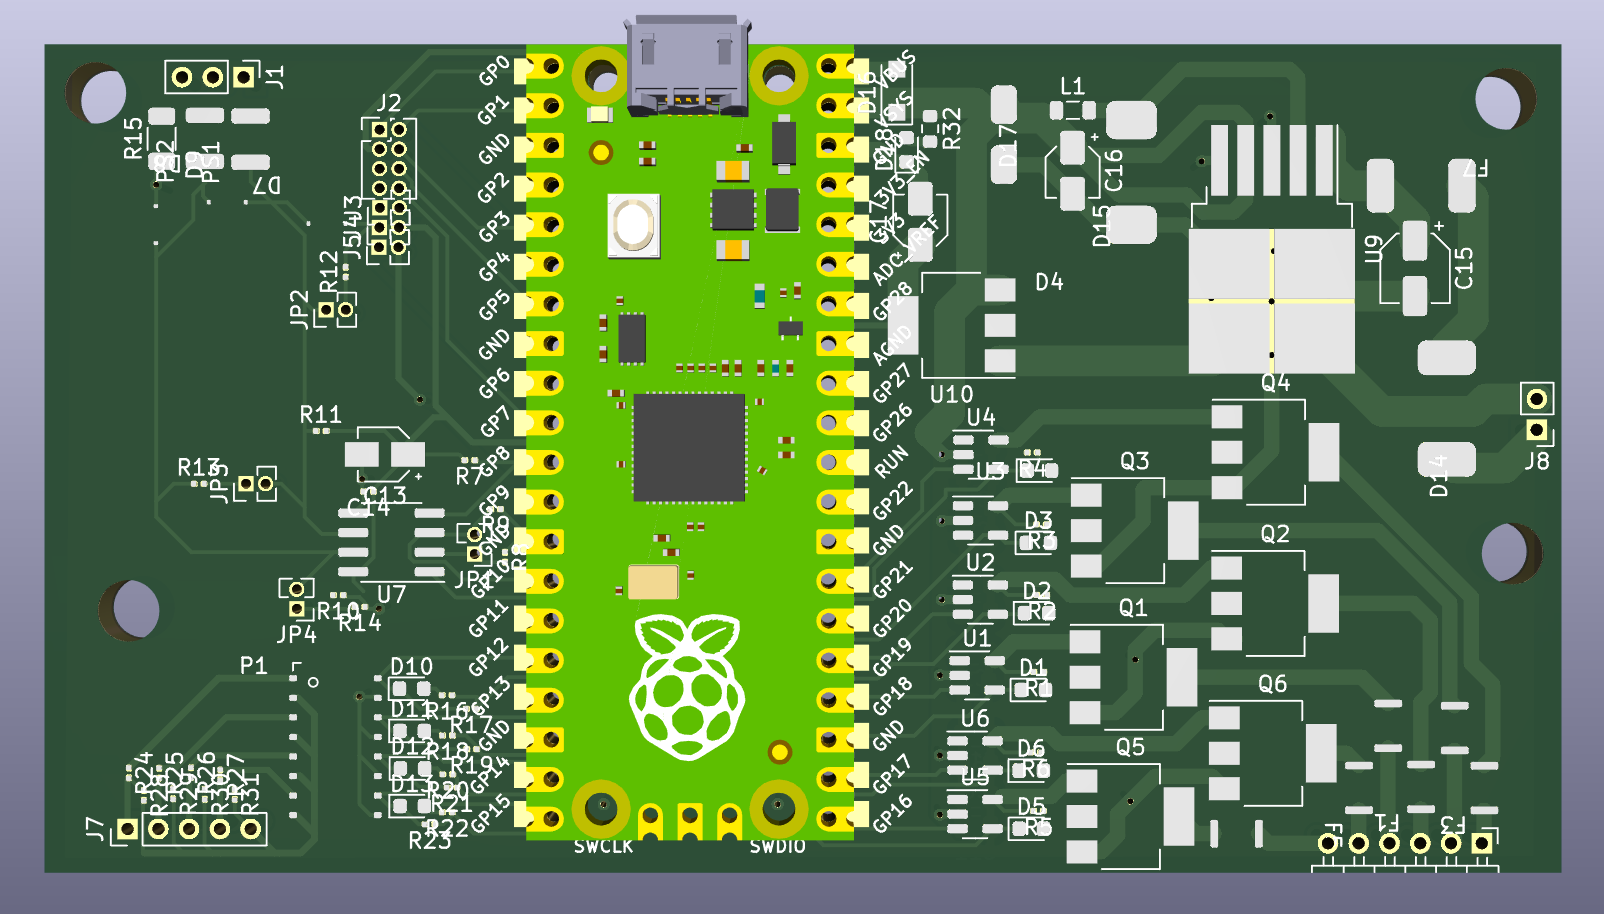
\includegraphics[width=0.8\linewidth]{fig/piaa3d.png}
    \caption{Vista 3D de PIAA.}
    \label{fig:piaa3d}
\end{figure}

\begin{figure}[htb]
    \centering
    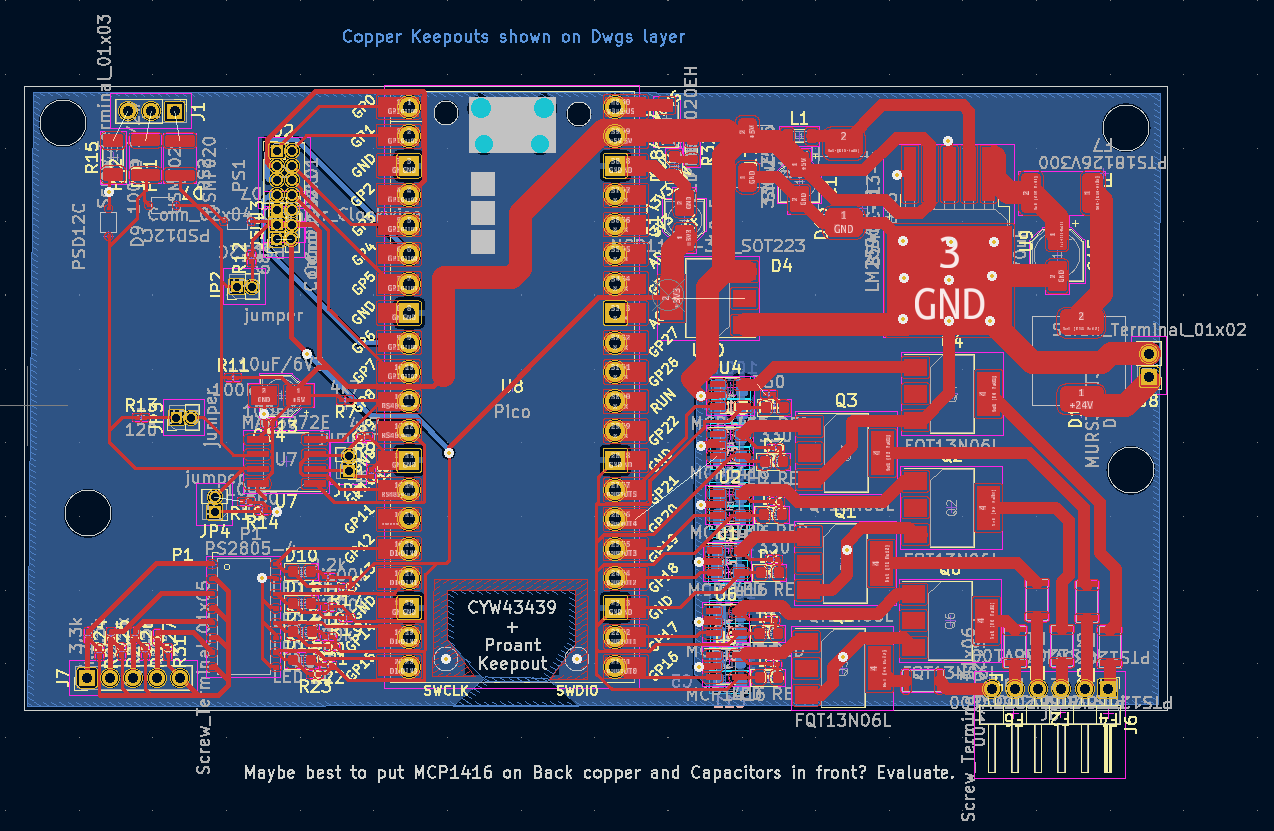
\includegraphics[width=0.8\linewidth]{fig/piaa_layout.png}
    \caption{Layout de pistas de la PIAA.}
    \label{fig:layoutpiaa}
\end{figure}

\clearpage

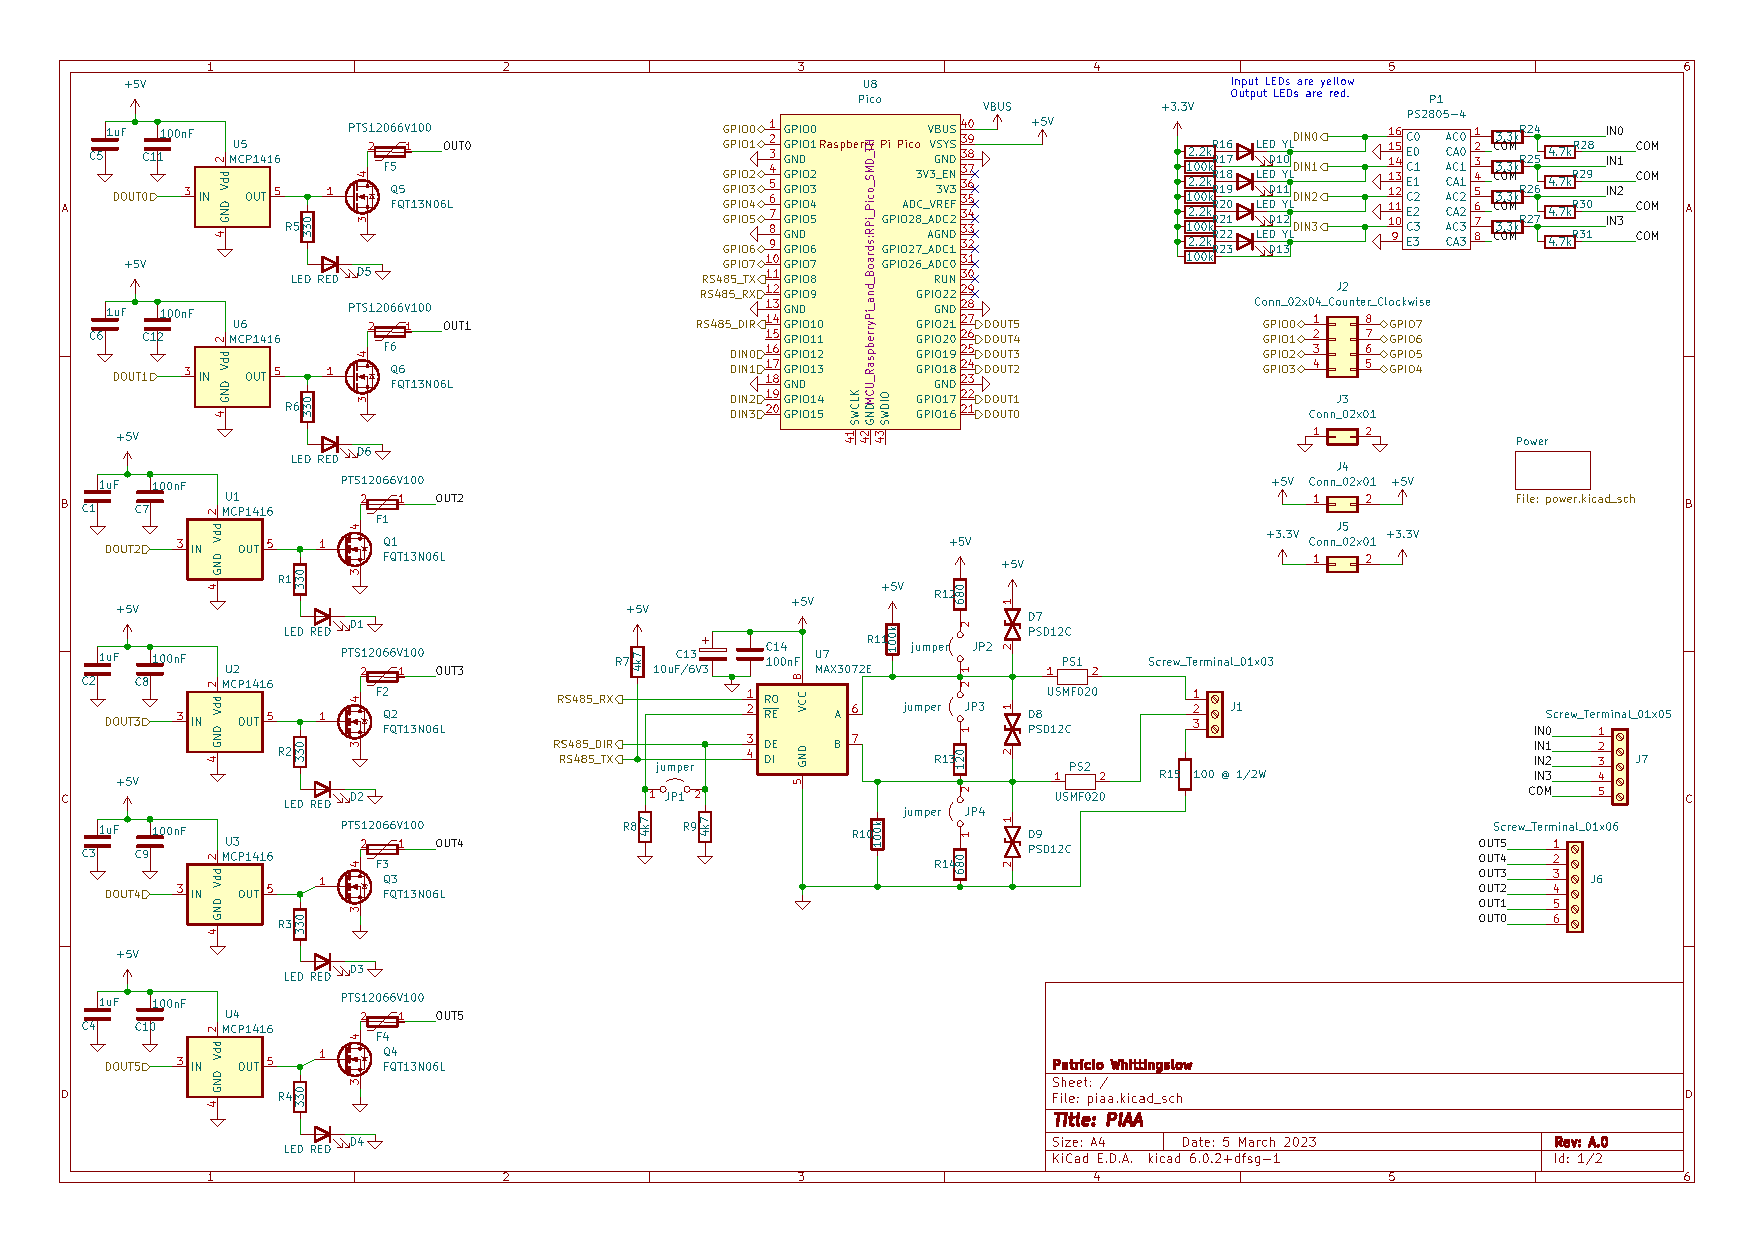
\includepdf[angle=90, page=1]{pdf/piaa_rev0.0.0.pdf}
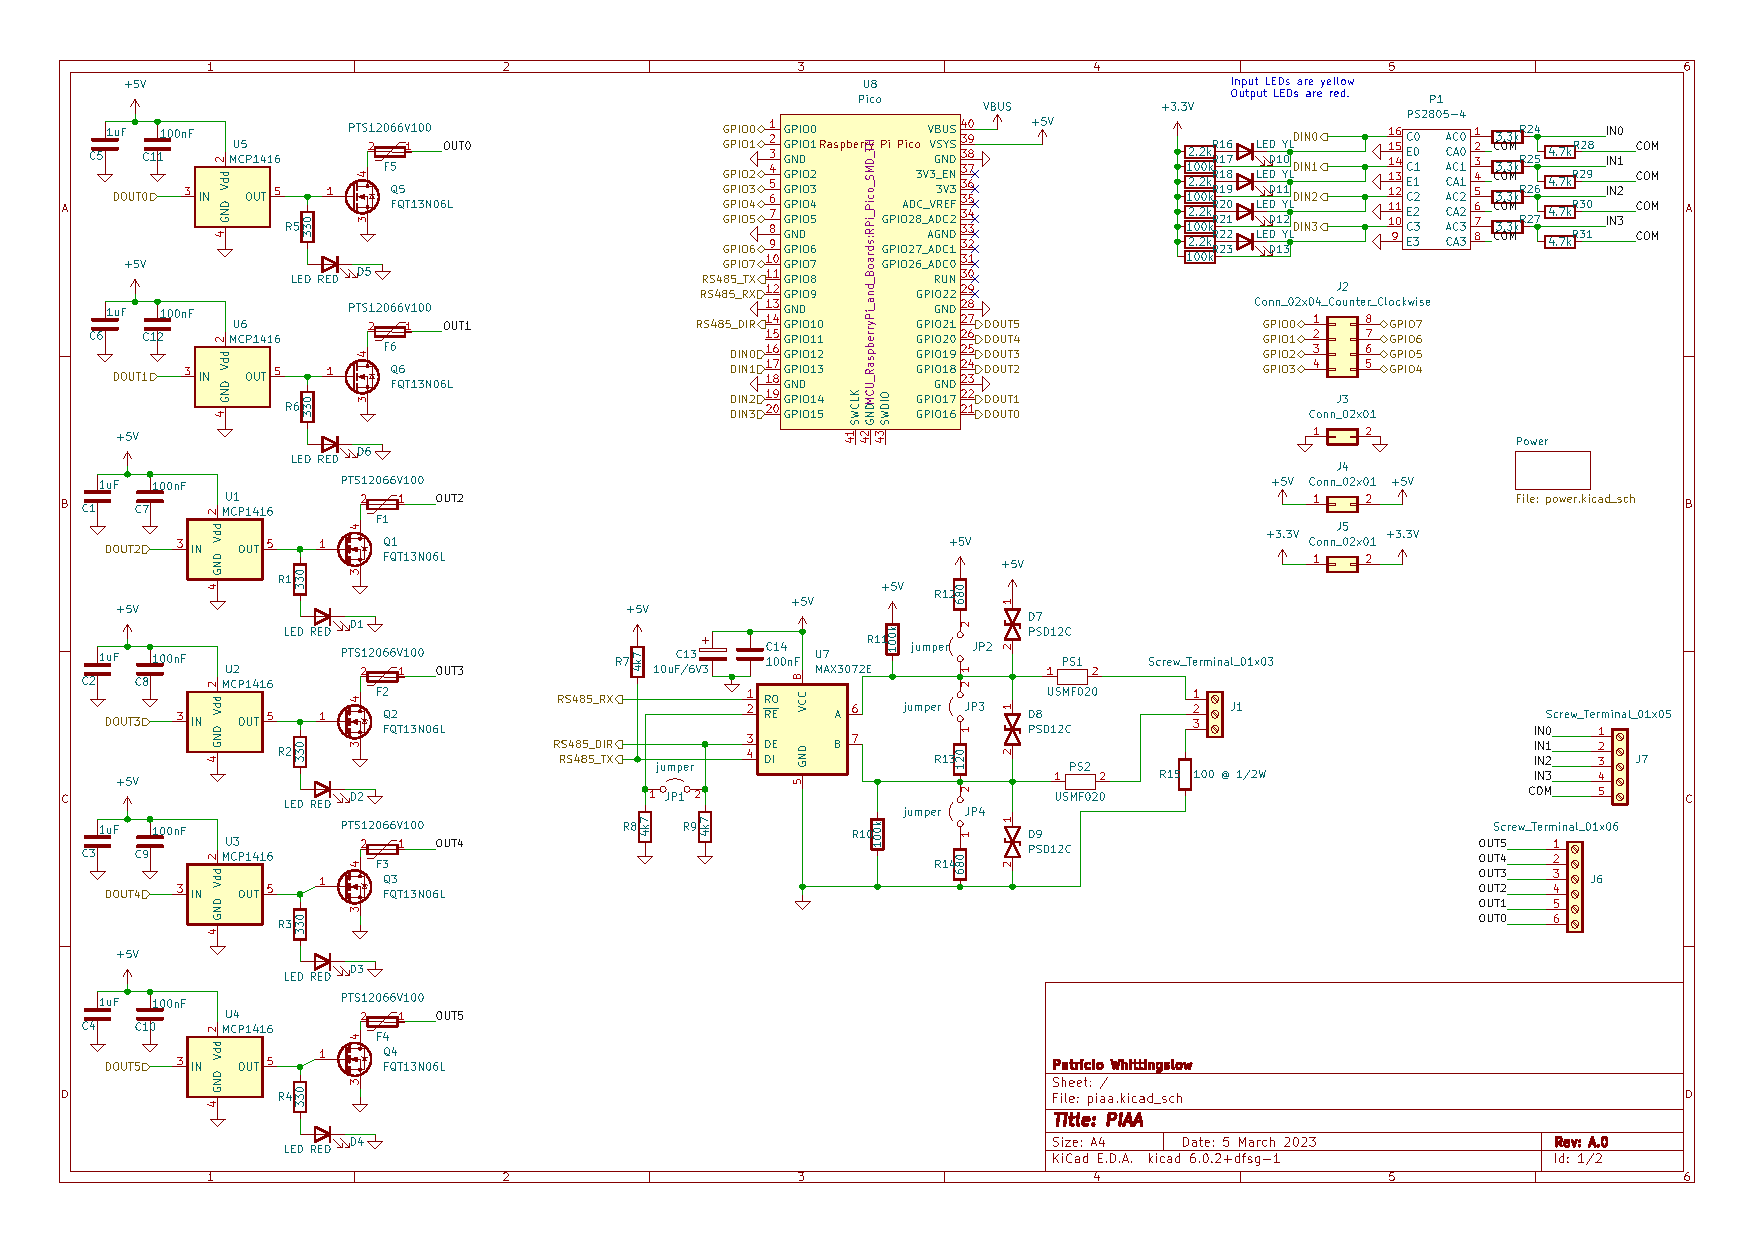
\includepdf[angle=90, page=2]{pdf/piaa_rev0.0.0.pdf}
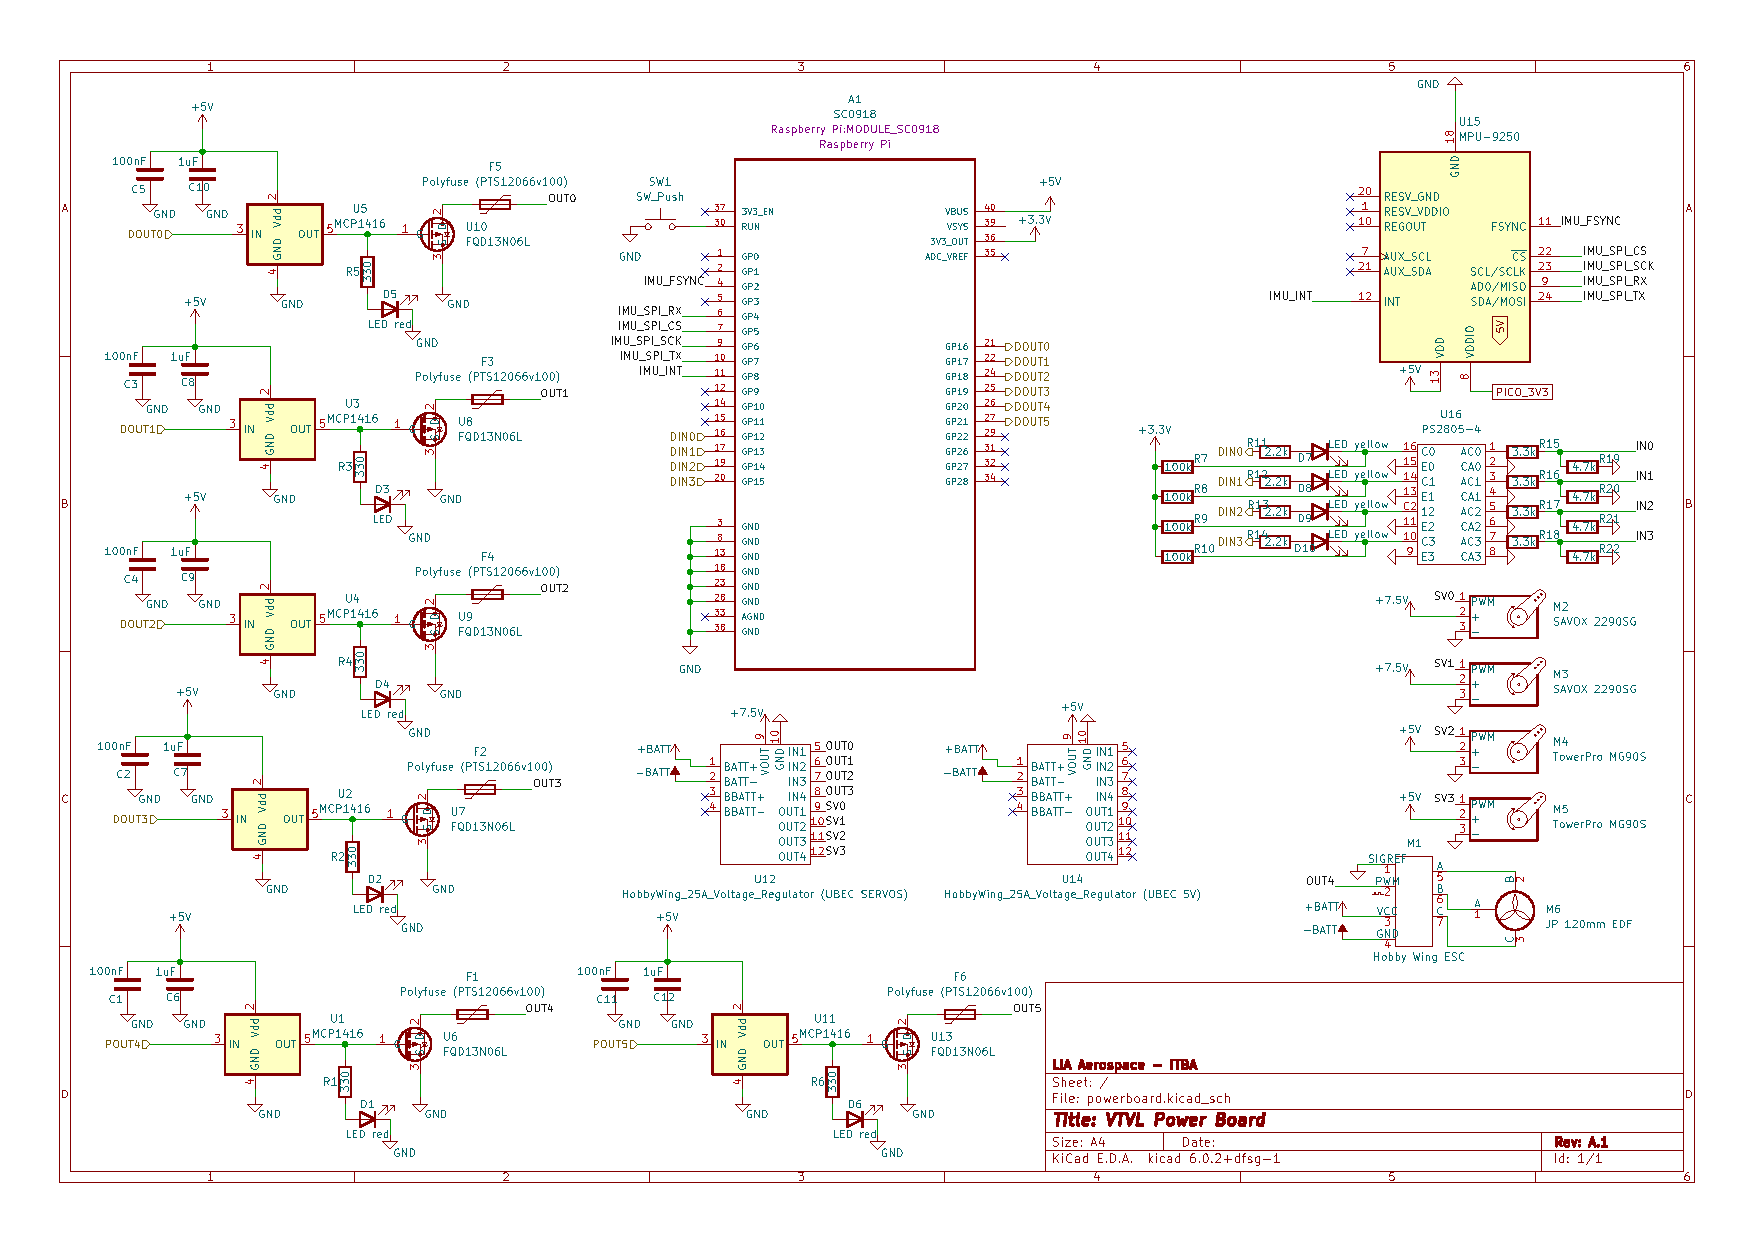
\includepdf[angle=90, page=1]{pdf/vtvlpowerboard.pdf}
\subsection{Contexto de pandemia}
Las medidas tomadas durante la pandemia por el gobierno fueron estrictas e influenció a todo tipo de acción que se quiso tomar. Durante el primer año de pandemia no nos pudimos reunir físicamente para discutir ideas de diseño, lo cual dificultó el avance físico del proyecto como así también la toma de decisiones y la comunicación entre partes, crucial en el inicio de todos proyectos de ingeniería.
El presente trabajo fue realizado por dos integrantes separados a 2000km de distancia, excluyendo el ensamblaje que fue realizado en el 2021 en las instalaciones de \gls{lia} una vez que se pudo coordinar una reunión presencial entre los participantes del proyecto.
\medskip

Una de las mayores complicaciones que se tuvo fue la compra de
componentes, además de la fabricación, que se vio afectada, por las políticas cambiantes de
nuestro país con respecto a la compra y la entrada de productos importados a suelo argentino.
Incluso la compra y llegada de los productos fue un motivo de festejo luego de un largo y complicado trayecto.
